\documentclass{standalone}
\usepackage{tikz}
\usetikzlibrary{automata,positioning}

\begin{document}
  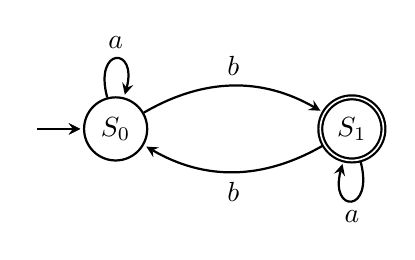
\begin{tikzpicture}[%
    >=stealth,
    shorten >=1pt,
    node distance=3cm,
    on grid,
    auto,
    state/.append style={minimum size=2em},
    thick
  ]
    \node[state, initial, initial text = {}] (A) {$S_0$};
    \node[state] (B) [accepting, right of=A] {$S_1$};

    \path[->] (A) +(-1,0) edge (A)
              (A)         edge [loop above]  node {$a$} (A)
              (A)         edge [bend left] node {$b$} (B)
              (B)         edge [loop below]  node {$a$} (B)
              (B)         edge [bend left] node {$b$} (A);
  \end{tikzpicture}
\end{document}